In this section, we evaluated our proposed method against other methods in the literature. From previous research about fault diagnosis in WSNs, we selected Support Vector Machine(SVM), Deep Belief Network \cite{Prasad2023}, and LSTM Classifier.

\subsection{Dataset}
For purpose of fault detection, we created an original dataset using data from NASA MERRA-2 reanalysis data (Temperature at 2 Meter) as substitution for measurements taken from a WSN. The data is collected from the North Vietnam region from a period of roughly 6 months. Another dataset used for performance evaluation is the Intel Lab Dataset. This dataset comprises readings from a network of 54 sensor nodes, specifically Mica2Dot devices, which were outfitted with environmental sensing capabilities. These nodes systematically captured time-stamped information relating to ambient conditions, including temperature, humidity, light levels, and the sensors' own voltage. The data acquisition process occurred at intervals of roughly 31 seconds for each sensor. The collection period for this particular dataset extended from late February 2004 through early April 2004 \cite{Intel2004}.

\subsection{Metrics}
To evaluate the performance of the proposed HiFiNet and compare it with other methods, several standard classification metrics are employed. These metrics are calculated based on the number of true positives (TP), false positives (FP), true negatives (TN), and false negatives (FN) for each class. In a multi-class classification problem, these are often computed for each class $c_i$ in a set of classes $C = \{c_1, c_2, \dots, c_K\}$.

Let \(TP_i\) be the number of true positives for class \(c_i\), \(FP_i\) be the number of false positives for class \(c_i\), \(FN_i\) be the number of false negatives for class \(c_i\), \(N\) be the total number of instances, \(N_i\) be the number of true instances belonging to class \(c_i\).

Accuracy measures the overall correctness of the classifier. It is the ratio of the number of correctly classified instances to the total number of instances.
\[\text{Accuracy} = \frac{\sum_{i=1}^{K} TP_i}{N}\]

Next, Recall measures the ability of the classifier to identify all positive instances of a particular class \(c_i\). It is the ratio of true positives for class \(c_i\) to the sum of true positives and false negatives for class \(c_i\).
\[\text{Recall}_i = \frac{TP_i}{TP_i + FN_i}\]
The weighted average recall is calculated as:
\[\text{Recall} = \sum_{i=1}^{K} \left( \frac{N_i}{N} \times \text{Recall}_i \right)\]

Precision measures the proportion of positively predicted instances for class \(c_i\) that were actually correct. It is calculated as the ratio of true positives for class \(c_i\) to the sum of true positives and false positives for class \(c_i\).
\[\text{Precision}_i = \frac{TP_i}{TP_i + FP_i}\]
The weighted average precision is computed as:
\[\text{Weighted Precision} = \sum_{i=1}^{K} \left( \frac{N_i}{N} \times \text{Precision}_i \right)\]

Finally, the F1-score is the harmonic mean of precision and recall for a class \(c_i\), providing a single score that balances both concerns.
\[\text{F1-score}_i = 2 \times \frac{\text{Precision}_i \times \text{Recall}_i}{\text{Precision}_i + \text{Recall}_i} \]
Similarly, the weighted average F1-score is calculated by:
\[\text{Weighted F1-score} = \sum_{i=1}^{K} \left( \frac{N_i}{N} \times \text{F1-score}_i \right)\]

\subsection{Evaluation Result}
Figure \ref{fig:INTEL_accuracy} represents the accuracy of each method with respect to the fault rate on Intel Lab data. HiFiNet outperforms existing algorithm, achieving higher accuracy across all fault injected rate measures. Furthermore, performance trends on the Intel Lab dataset indicate that while all methods experience a decline in accuracy as the fault injection rate increases, HiFiNet demonstrates greater robustness. For instance, as the fault rate escalates from 5\% to 20\%, HiFiNet's accuracy decreases from approximately 93.08\% to 88.8\%, a reduction of 4.28 percentage points. In contrast, the LSTM classifier's accuracy drops by about 12.6 percentage points (from 91.4\% to 78.8\%), SVM by 16.5 percentage points (from 87.1\% to 70.6\%), and DBN by 14.6 percentage points (from 84.6\% to 70.0\%) under the same conditions. This suggests that HiFiNet degrades less significantly with an increasing percentage of faults.

\begin{figure}
  \centering
    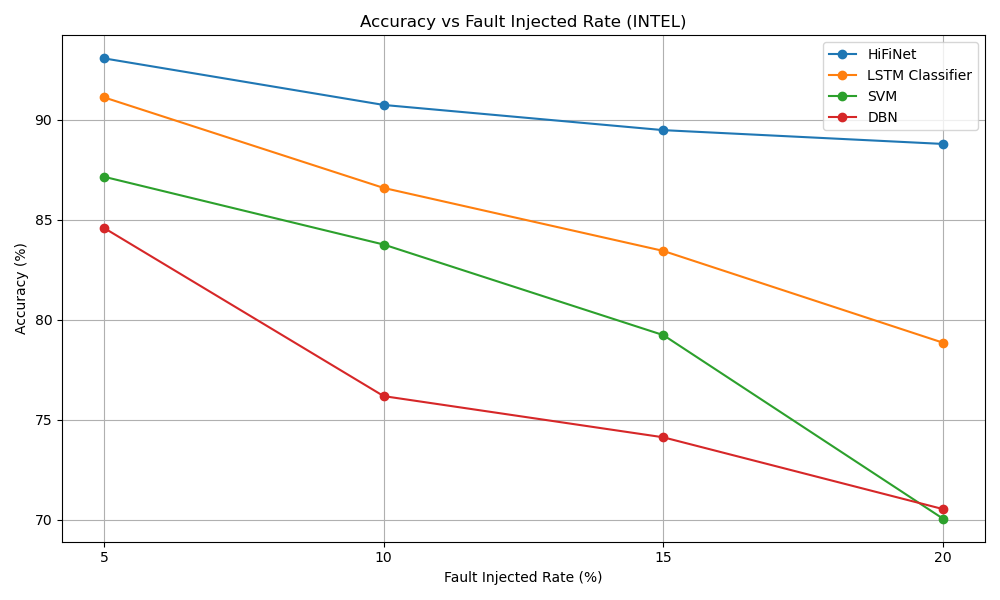
\includegraphics[width=0.8\textwidth]{images/INTEL_accuracy.png}
    \caption{Accuracy versus Fault Rate in the Intel Lab dataset.}
    \label{fig:INTEL_accuracy}
\end{figure}

Similarly, figure \ref{fig:MERRA-2_accuracy} represents the accuracy of each method with respect to the fault rate on MERRA-2 data. HiFiNet also exhibits notable improvement on MERRA-2 dataset and less performance degradation as fault rate increase. It was also observed that models generally achieved higher accuracy on the MERRA-2 dataset compared to the Intel Lab dataset. This difference may be attributed to the data characteristics; the MERRA-2 dataset, with its one-hour sampling interval, tends to exhibit clearer cyclical patterns which can aid in distinguishing normal behavior from faulty data. The Intel Lab dataset, with a five-minute interval, contains more rapid fluctuations, potentially making it more challenging to model normal variations and identify anomalies.

\begin{figure}
  \centering
    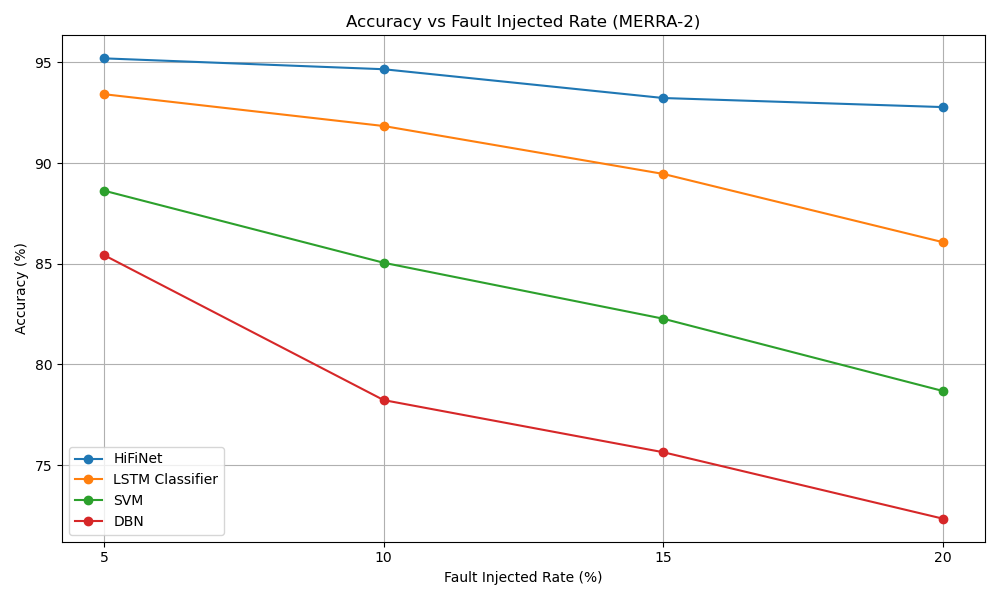
\includegraphics[width=0.8\textwidth]{images/MERRA-2_accuracy.png}
    \caption{Accuracy versus Fault Rate in the Intel Lab dataset.}
    \label{fig:MERRA-2_accuracy}
\end{figure}

A detailed breakdown of performance metrics, including accuracy, F1-score, recall, and precision, for the MERRA-2 dataset is provided in Table \ref{tab:merra2_results}. The results presented in confirm the superior performance of HiFiNet on the MERRA-2 dataset across all evaluated metrics and fault injection levels. At fault injection rates of 5\,\%, 10\,\%, 15\,\%, and 20\,\%, HiFiNet’s F1‐scores are 94.70\,\%, 94.49\,\%, 93.12\,\%, and 92.64\,\%, respectively, illustrating that it sustains an excellent balance between identifying true faults and avoiding false alarms. In comparison, the LSTM classifier’s F1‐score gradually diminishes from 92.04 \% (5 \%) to 90.93 \% (10 \%), 88.68 \% (15 \%), and 85.37 \% (20 \%), demonstrating that it both misses an increasing number of true faults and generates more false positives as the fault rate rises. The SVM’s performance degrades even more steeply: its F1‐scores drop from 86.62 \% (5 \%) to 81.68 \% (10 \%), 79.64 \% (15 \%), and 75.43 \% (20 \%).

\begin{table}[H]
\centering
\label{tab:merra2_results}
\begin{tabular*}{\textwidth}{@{\extracolsep{\fill}}lrrrr}
\hline
\multicolumn{5}{l}{Accuracy} \\
& 5\% & 10\% & 15\% & 20\% \\
\hline
HiFiNet & 95.20 & 94.66 & 93.23 & 92.78 \\
LSTM Classifier & 93.42 & 91.84 & 89.46 & 86.07 \\
SVM & 88.63 & 85.05 & 82.27 & 78.68 \\
DBN & 85.34 & 78.23 & 75.64 & 72.34 \\
\hline
\multicolumn{5}{l}{F1-score} \\
& 5\% & 10\% & 15\% & 20\% \\
\hline
HiFiNet & 94.70 & 94.49 & 93.12 & 92.64 \\
LSTM Classifier & 92.04 & 90.93 & 88.68 & 85.37 \\
SVM & 86.62 & 81.68 & 79.64 & 75.43 \\
DBN & NA & NA & NA & NA \\
\hline
\multicolumn{5}{l}{Recall} \\
& 5\% & 10\% & 15\% & 20\% \\
\hline
HiFiNet & 95.20 & 94.66 & 93.23 & 92.78 \\
LSTM Classifier & 93.42 & 91.84 & 89.46 & 86.07 \\
SVM & 88.99 & 85.05 & 82.71 & 78.68 \\
DBN & NA & NA & NA & NA \\
\hline
\multicolumn{5}{l}{Precision} \\
& 5\% & 10\% & 15\% & 20\% \\
\hline
HiFiNet & 95.21 & 94.52 & 93.55 & 92.89 \\
LSTM Classifier & 92.10 & 91.53 & 89.35 & 85.55 \\
SVM & 86.95 & 82.78 & 81.62 & 79.20 \\
DBN & NA & NA & NA & NA \\
\hline
\end{tabular*}
\caption{Performance metrics on the MERRA-2 dataset with varying fault injection rates. Values are in percentage (\%).}
\end{table}

